\chapter{Results} \label{chapResults}
\section{Structure from motion on drone forest images}


\begin{figure}[h]
    \subfloat{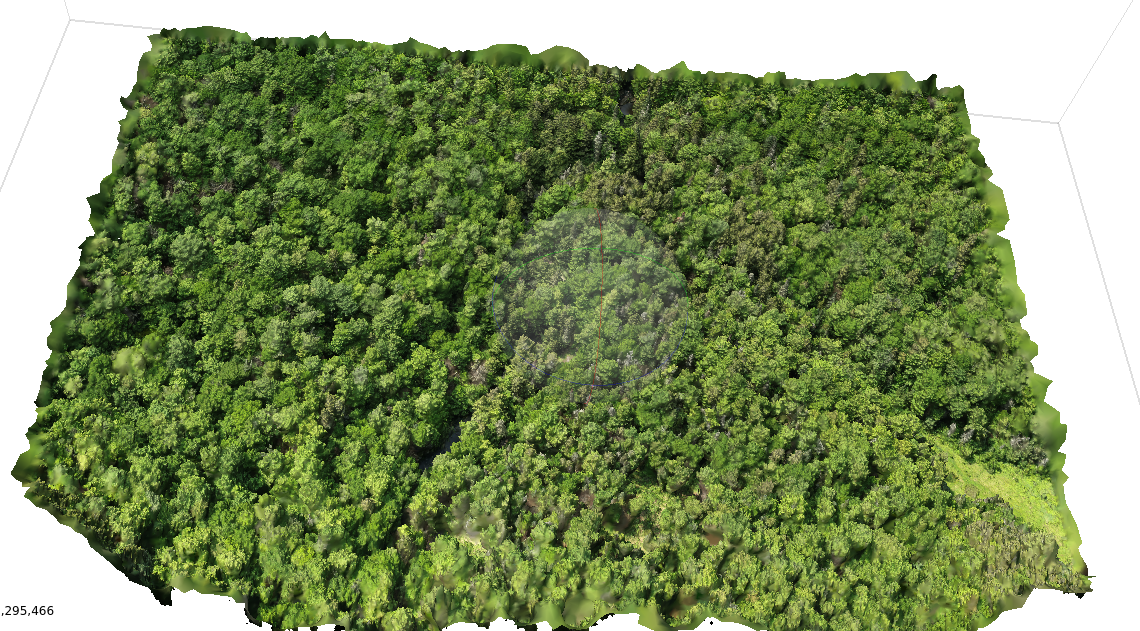
\includegraphics[width=0.45\textwidth]{figs/results/geometric_understanding/stowe_anew_collect_000_zoomed_out.png}}
    \hfill
    \subfloat{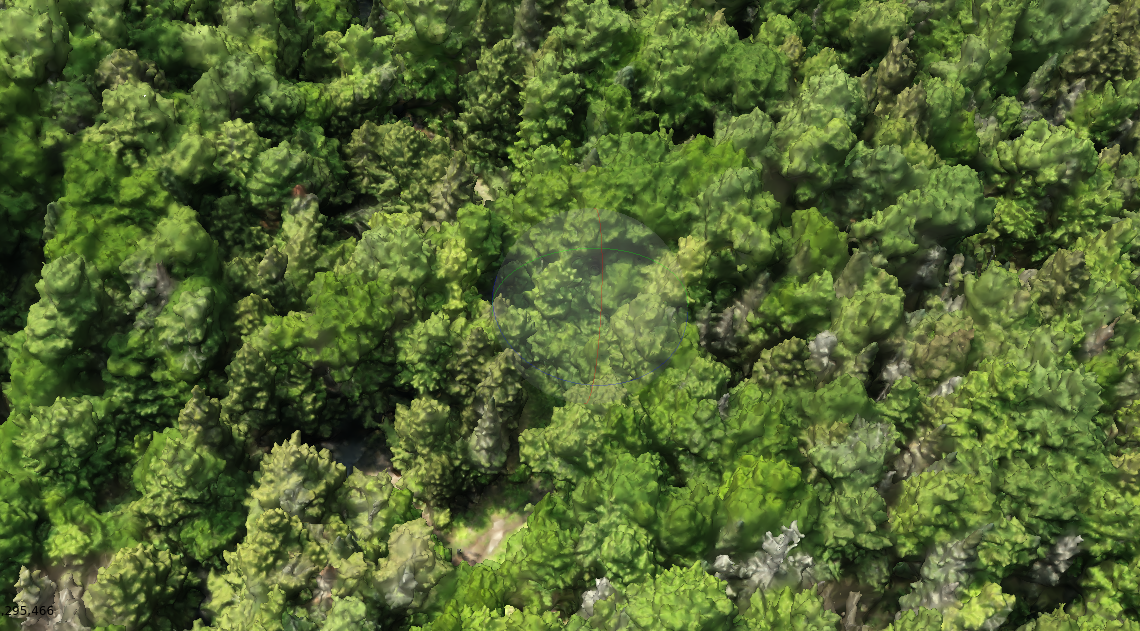
\includegraphics[width=0.45\textwidth]{figs/results/geometric_understanding/stow_anew_collect_000_zoomed_in.png}}\\
        
    \subfloat{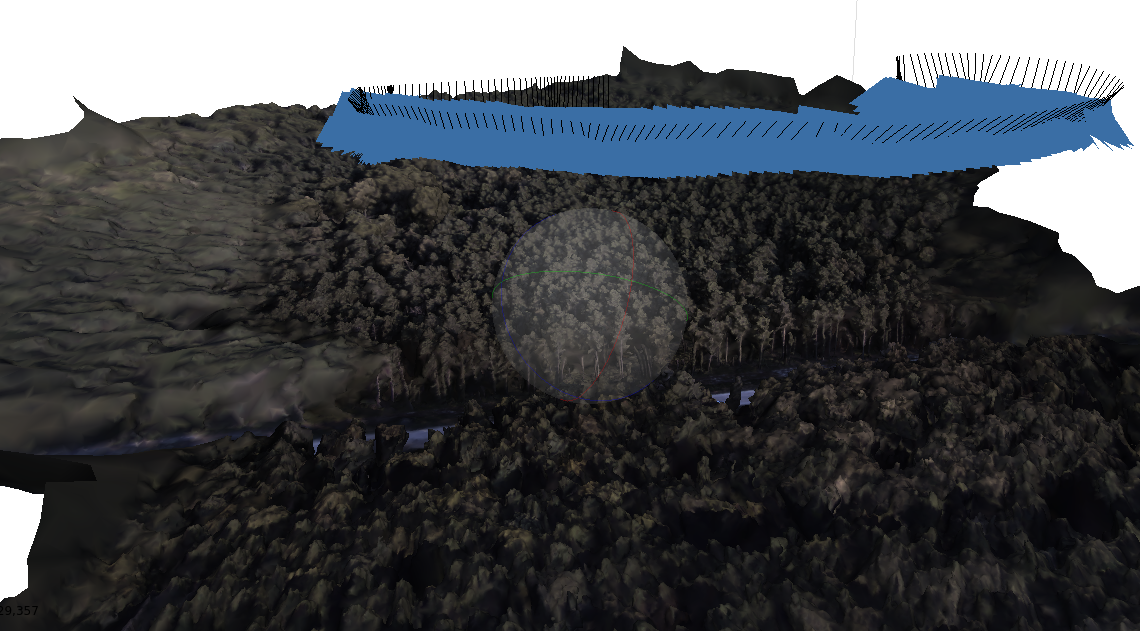
\includegraphics[width=0.45\textwidth]{figs/results/geometric_understanding/burn_zoomed_out.png}}
    \hfill
    \subfloat{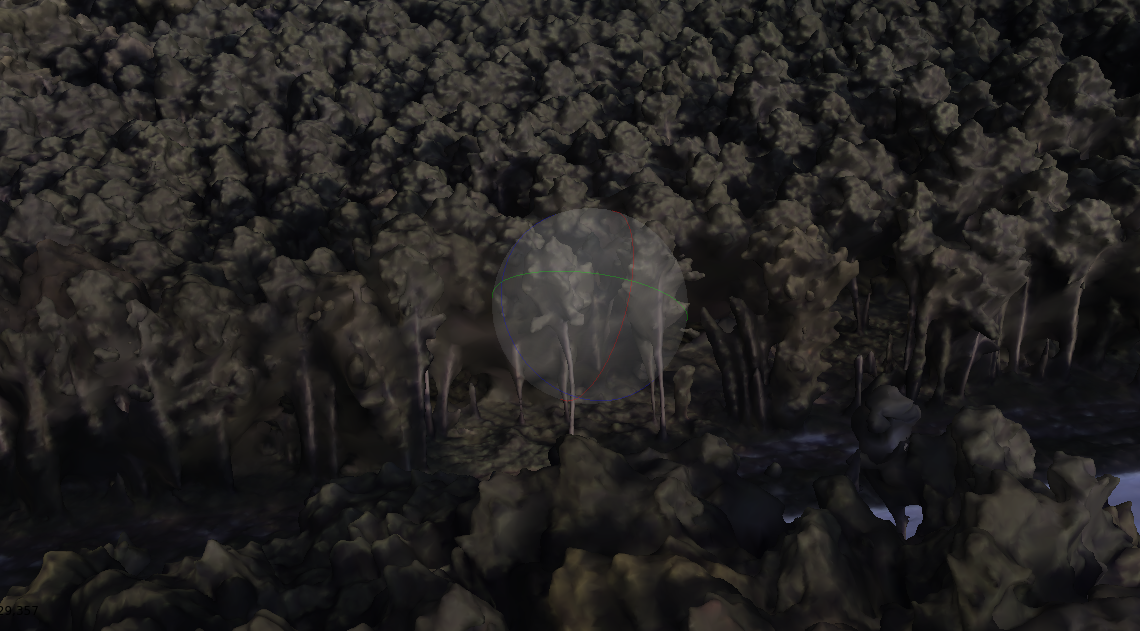
\includegraphics[width=0.45\textwidth]{figs/results/geometric_understanding/burn_zoomed_in.png}}\\
    
    \subfloat{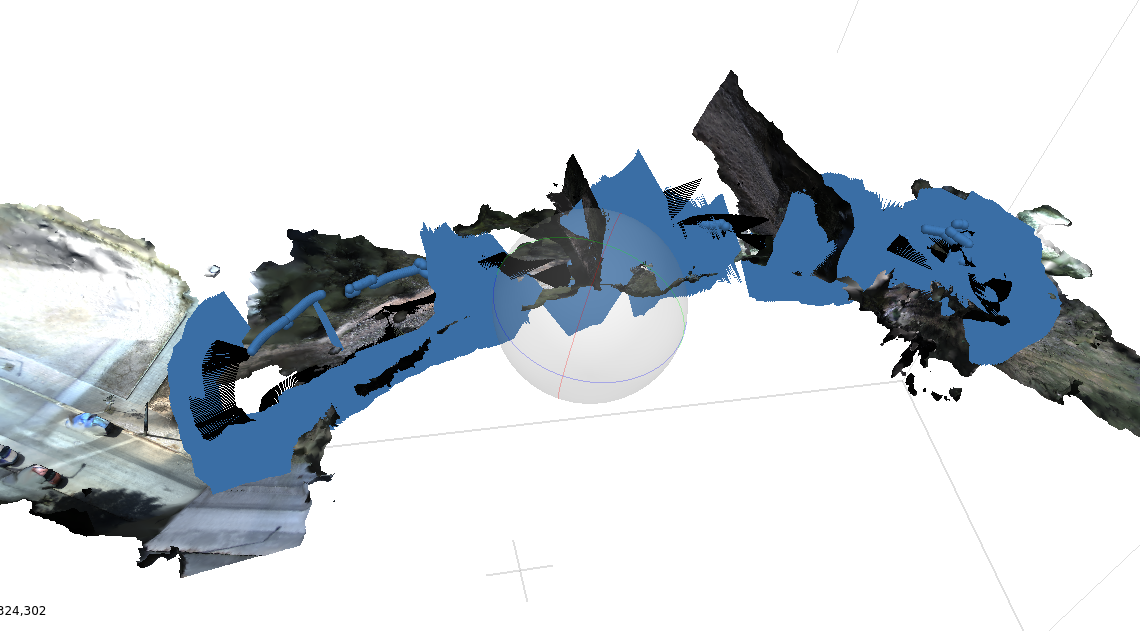
\includegraphics[width=0.45\textwidth]{figs/results/geometric_understanding/coimbra_zoomed_out.png}}
    \hfill
    \subfloat{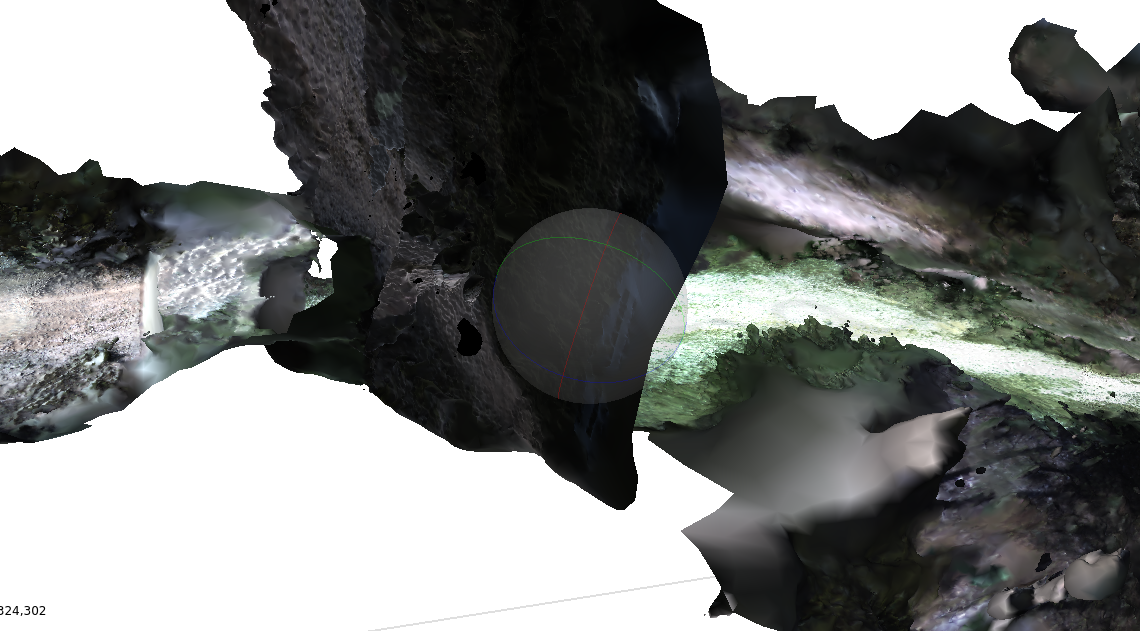
\includegraphics[width=0.45\textwidth]{figs/results/geometric_understanding/coimbra_zoomed_in.png}}
    \caption{3D reconstructions using Agisoft Metashape on three different environments. The full map is shown to the left and a zoomed-in inset is shown to the right.}
    \label{fig:results:sfm}
\end{figure}

A key first step in all the approaches we used is understanding the structure of the forest scene. In this work, we primarily leveraged structure from motion to obtain mesh representations of the environment. We found that the quality of the results depended heavily on the flight pattern that was used to collect the data. Automated over canopy lawnmower surveys performed the best and manual over canopy flights were slightly worse because of the lower density of observations and decreased consistency. Under canopy manual data collects had the worst results and often failed to properly identify the pose of many of the cameras. Results can be seen in Figure \ref{fig:results:sfm}.


\begin{figure*}[h!]
   \centering
   %----primera subfigura----
   \subfloat[]{
        \label{fig:metashape_cloud_baseline}         %% Etiqueta para la primera subfigura
        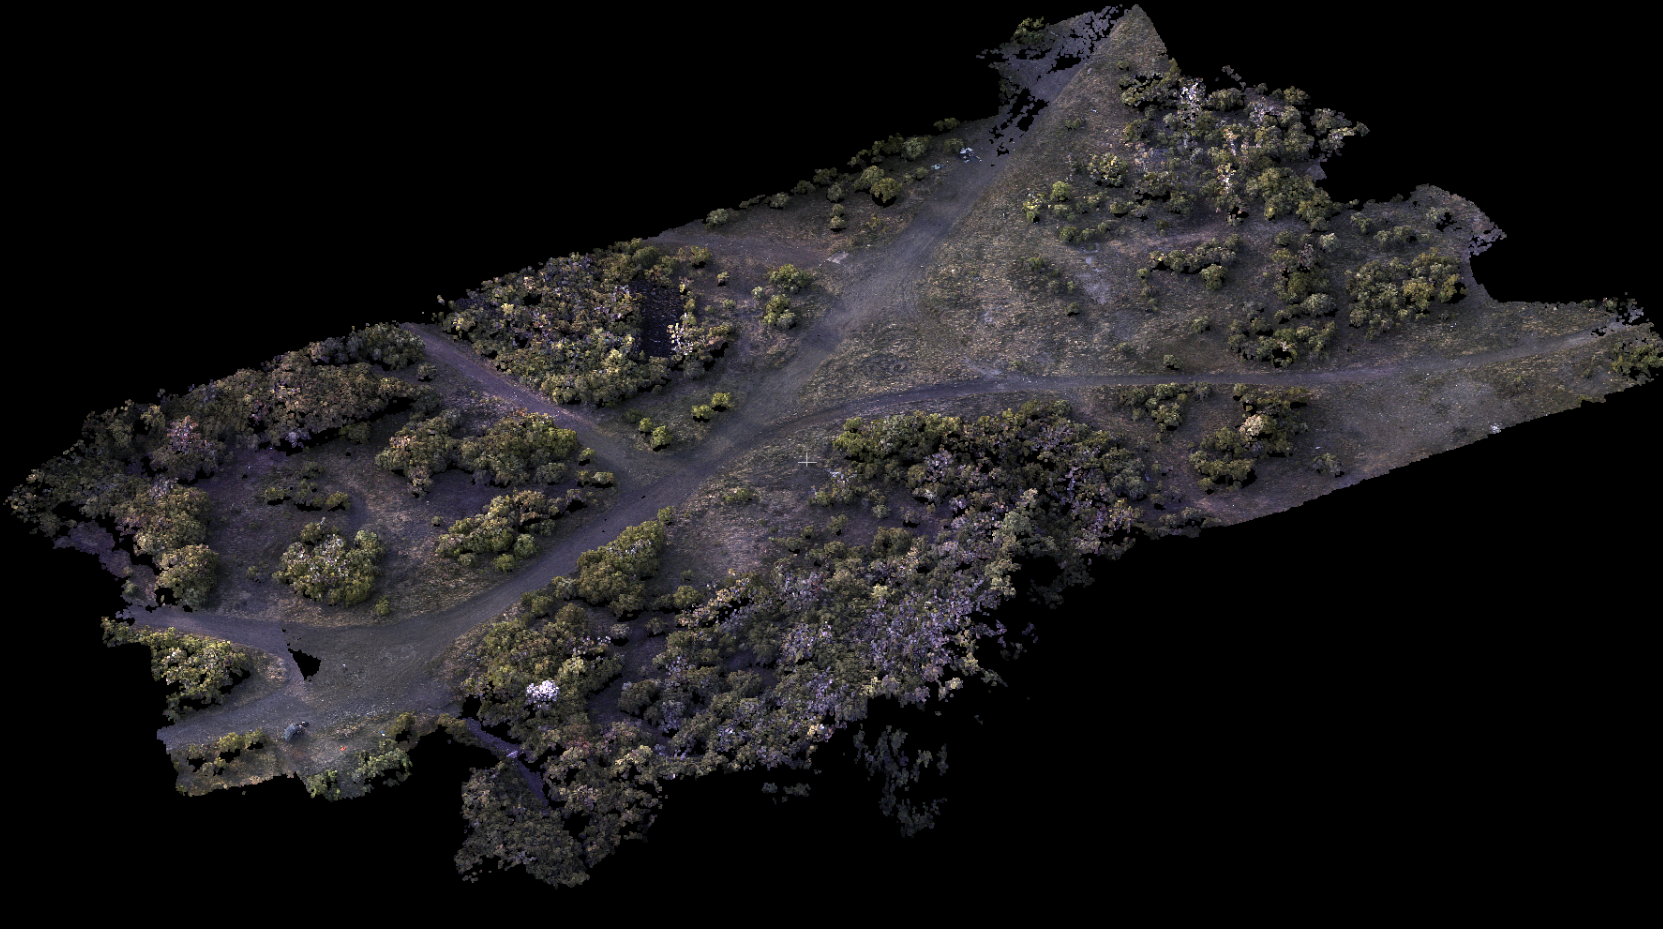
\includegraphics[width=0.465\textwidth]{figs/results/geometric_understanding/metashape_cloud_v3.png}}
   %\hspace{0.1\linewidth}
   \subfloat[]{
        \label{fig:slam_orig_1}         %% Etiqueta para la segunda subfigura
        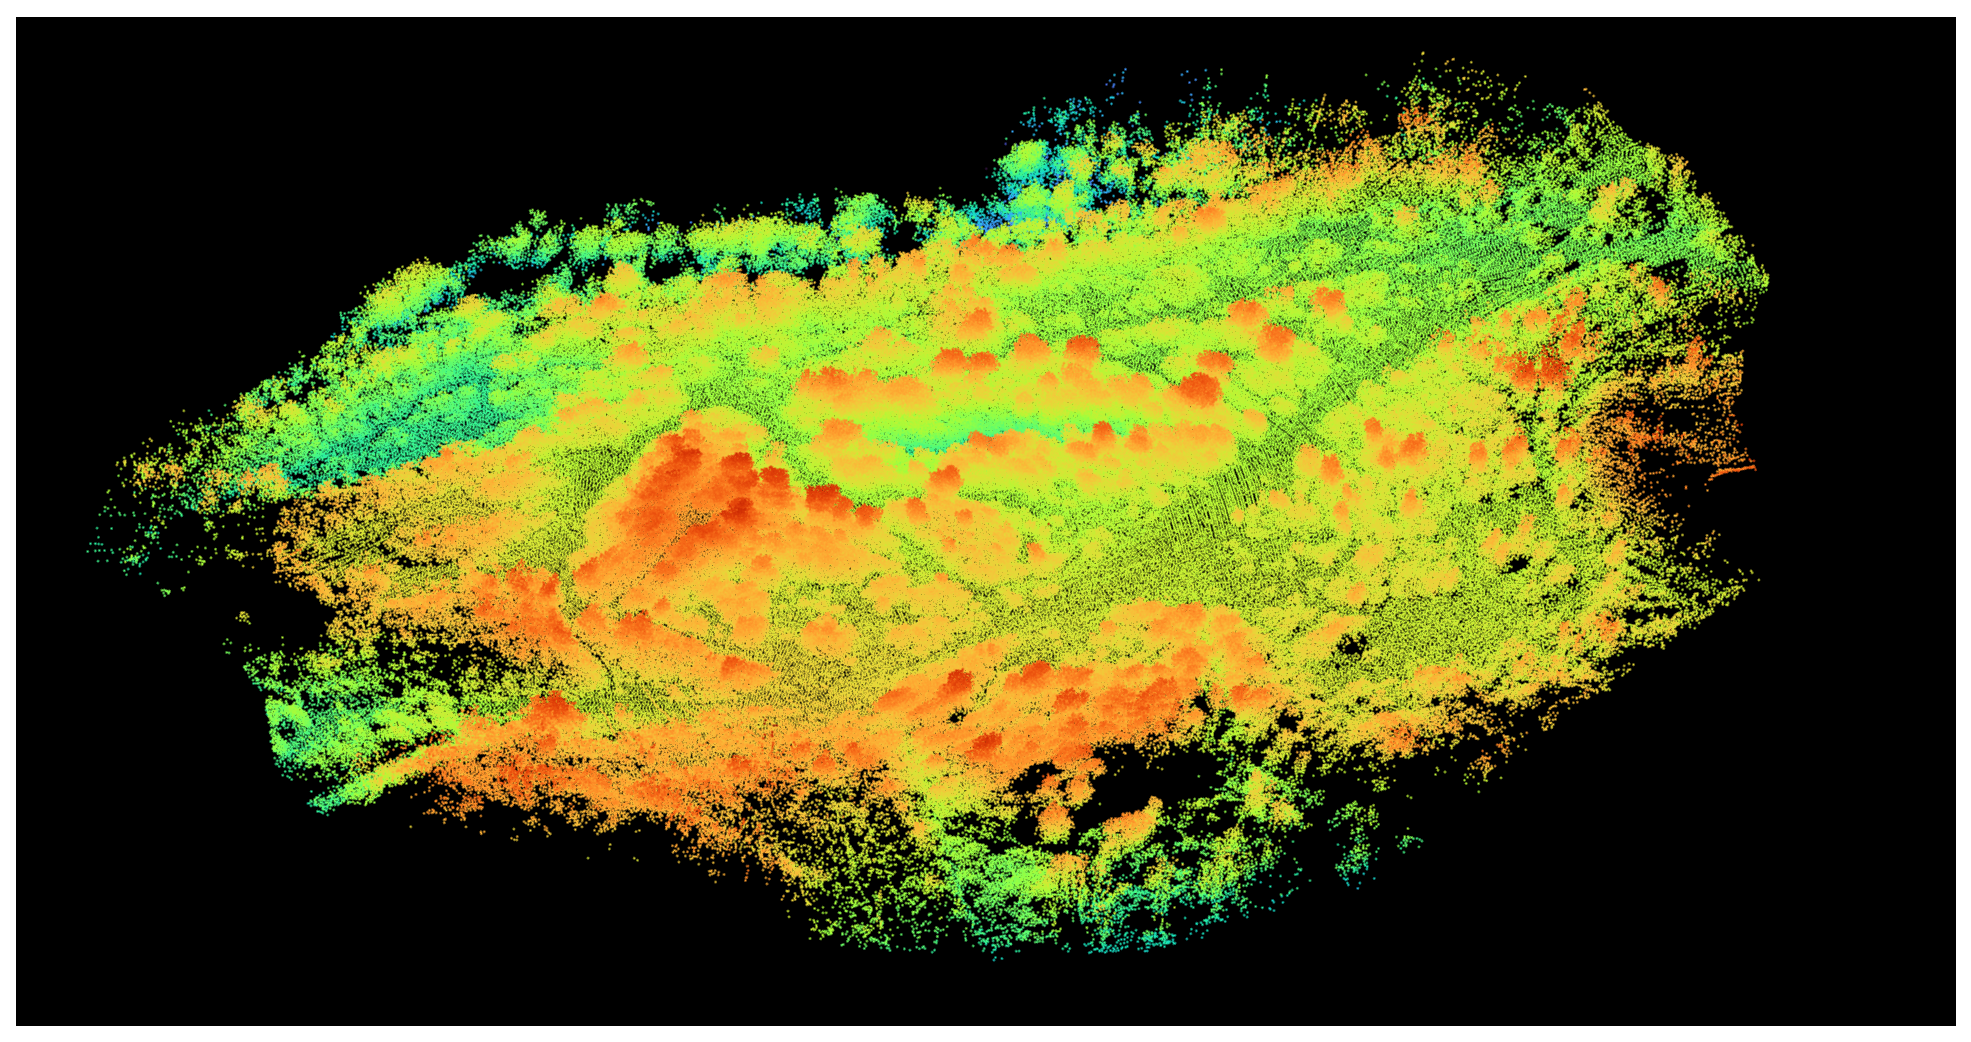
\includegraphics[width=0.5\textwidth]{figs/results/geometric_understanding/slam_ptCloud.eps}}\\%\\[20pt]   
   \subfloat[]{
        \label{fig:slam_hausdorff}         %% Etiqueta para la segunda subfigura
        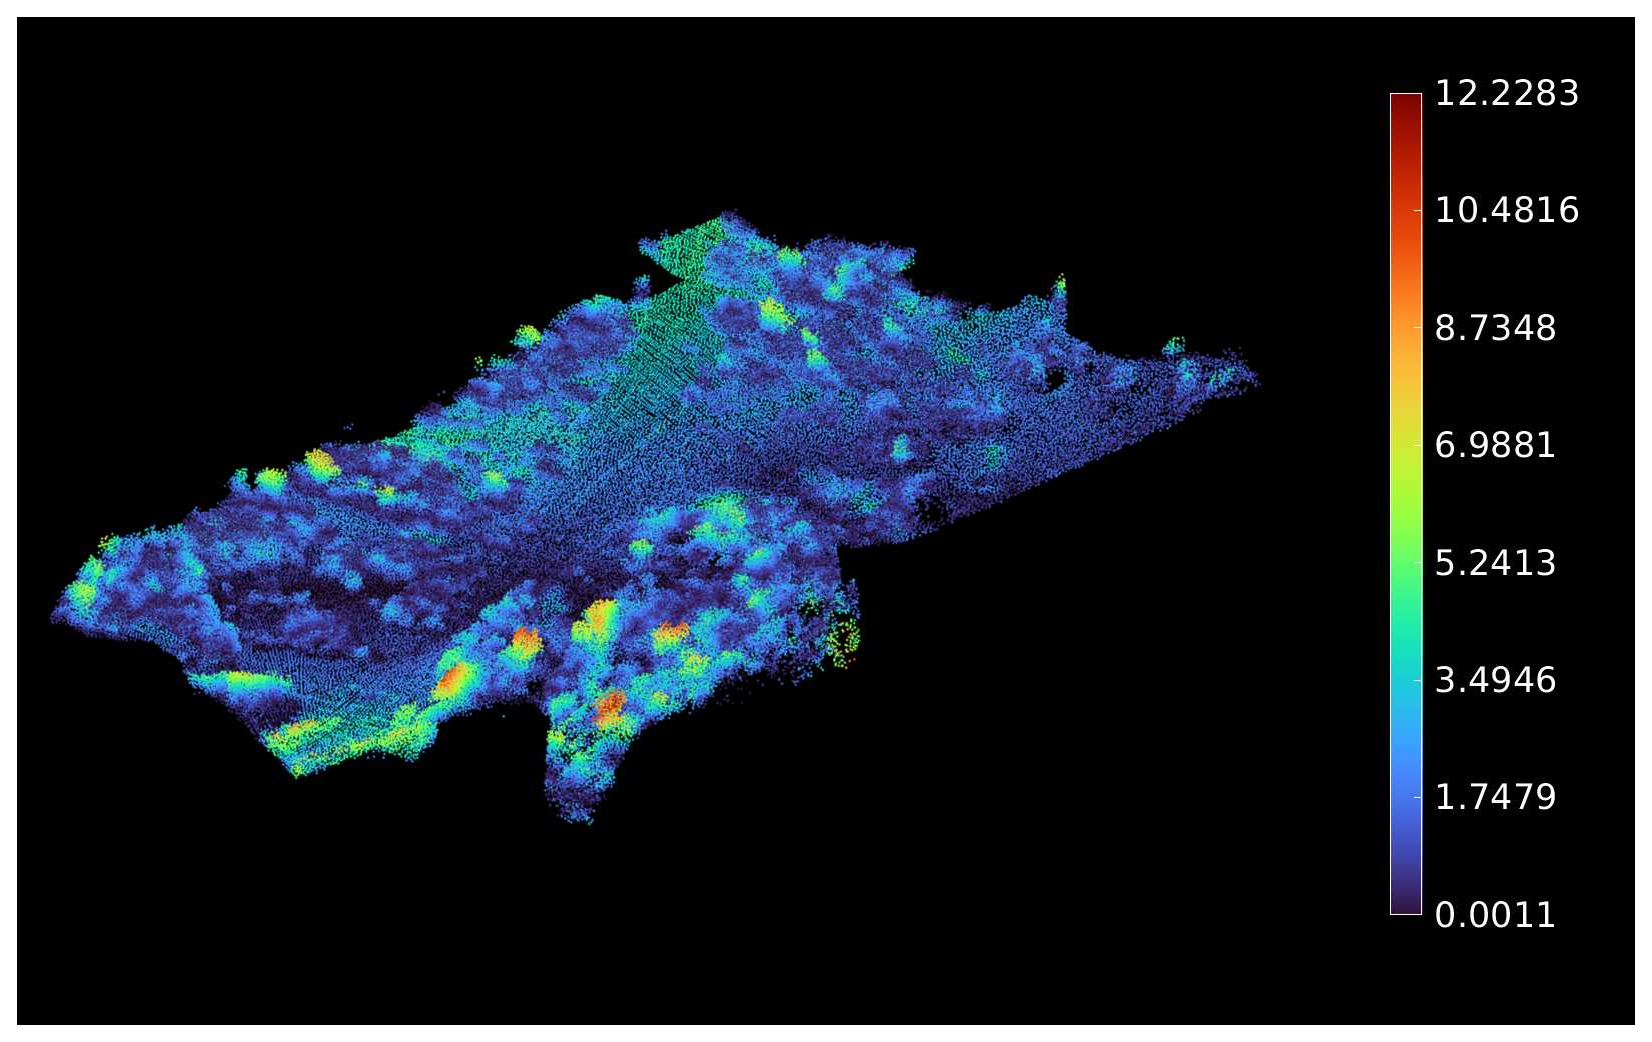
\includegraphics[width=0.5\textwidth]{figs/results/geometric_understanding/housedorff_distance.eps}}%\\[20pt]            
   \caption{Point cloud maps of the A) photogrammetry baseline, B) SLAM outcome. The two maps were compared using the Hausdorff distance, whose result is visualized as C) the SLAM map colored according to this metric. Note that the baseline and the SLAM clouds colormaps correspond to RGB and height values, respectively. Figure courtesy of Dr. Francisco Yandun.}
   \label{fig:results_mapping_slam}                %% Etiqueta para la figura entera
\end{figure*}

Properly exposing the images is an important consideration. This is generally addressed automatically by consumer hardware, but may require hand-tuning on a robotic research platfrom.

\section{Semantic mapping}



\subsection{Image segmentation}
We conduct two studies on semantic segmentation in a forestry environment.

Given the limited availability of real data and the labor-intensive nature of labeling to obtain ground truth, we explored the utility of models trained with simulated (\textit{synthetic}) data. We conducted three types of experiments: models trained solely with \textit{synthetic} data, models trained with real data (\textit{Setes Fontes}), and a mixture of both. For the last two cases, we trained with an increasing number of real images to evaluate the performance of the model with minimal real images. Thus, we conducted training experiments using (or adding) 7, 15, 21, 30, 60, 91, and 121 data points from the \textit{Setes Fontes} dataset. We trained for 10000 iterations and evaluated each model in 30 \textit{Setes Fontes} images not seen in the largest training split are used for evaluation and we replicate this experiment over five folds of the data. The three models are a fine-tuned implementation as the base networks were first trained with the \textit{CityScapes} dataset \cite{Cordts2016}.

\begin{figure}
    \centering
    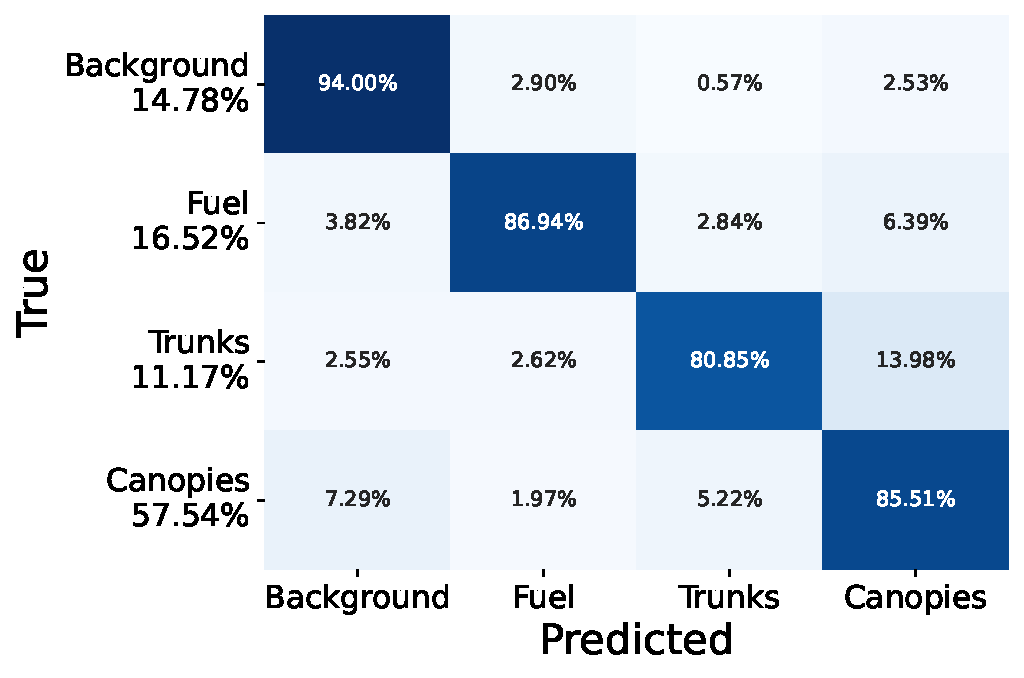
\includegraphics[width=0.7\columnwidth]{figs/results/semantic_segmentation/confusion_matrix.pdf} 
    \caption{Confusion matrix for the \textit{Setes Fontes} test datasets normalized per class with the true fraction of each class reported on the y axis labels.
    %Fuel is predicted fairly well, though it is fairly often confused for canopy, which is understandable given the visual similarity and the large fraction of canopy pixels.
    }
    \label{fig:semantics_confusion}
\end{figure}
\begin{figure}
   % First row
   \centering
    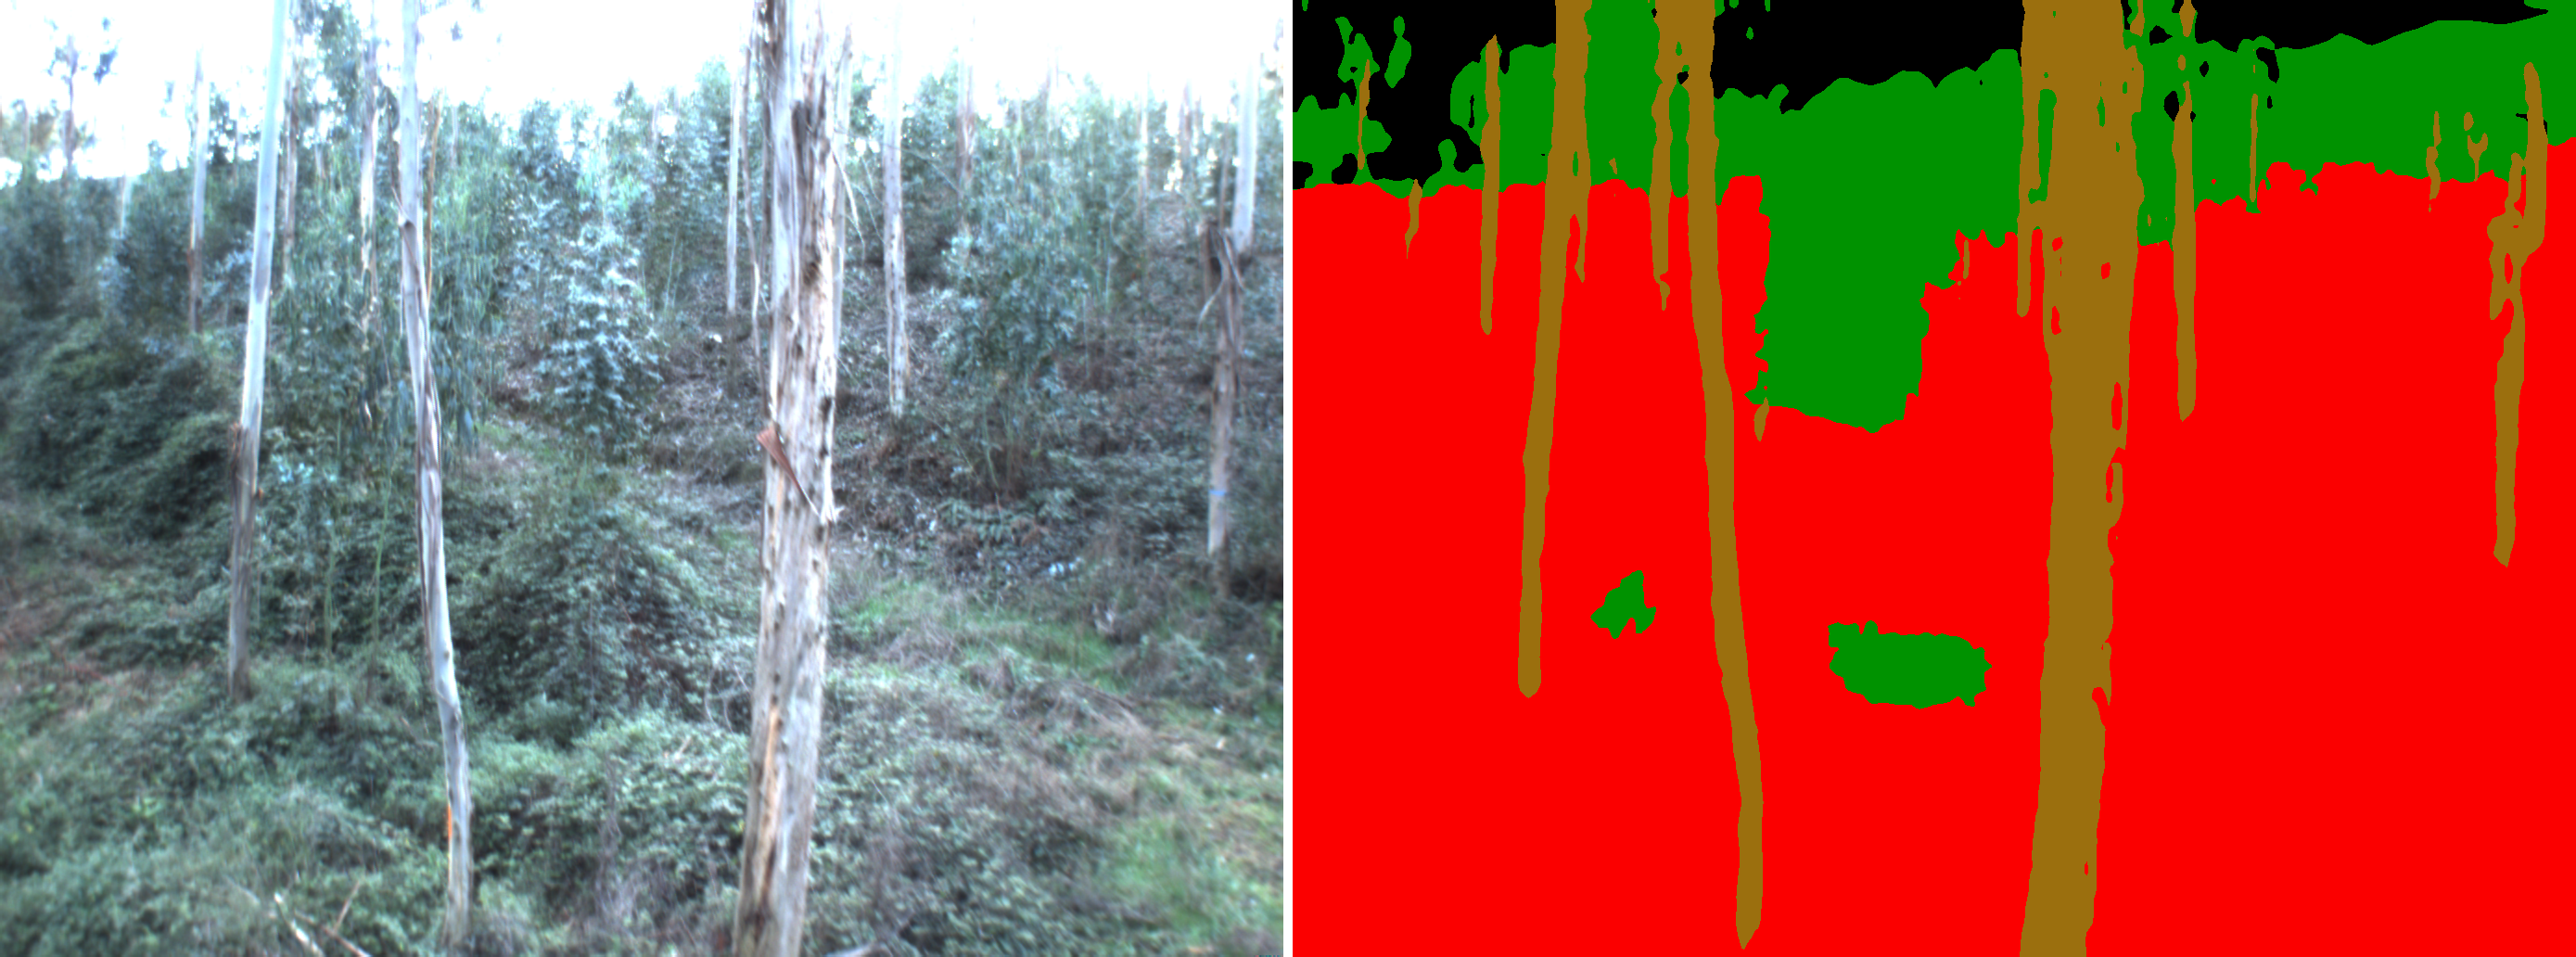
\includegraphics[width=\linewidth]{figs/results/semantic_segmentation/SeteFontes/qualatative_001400.png}  
    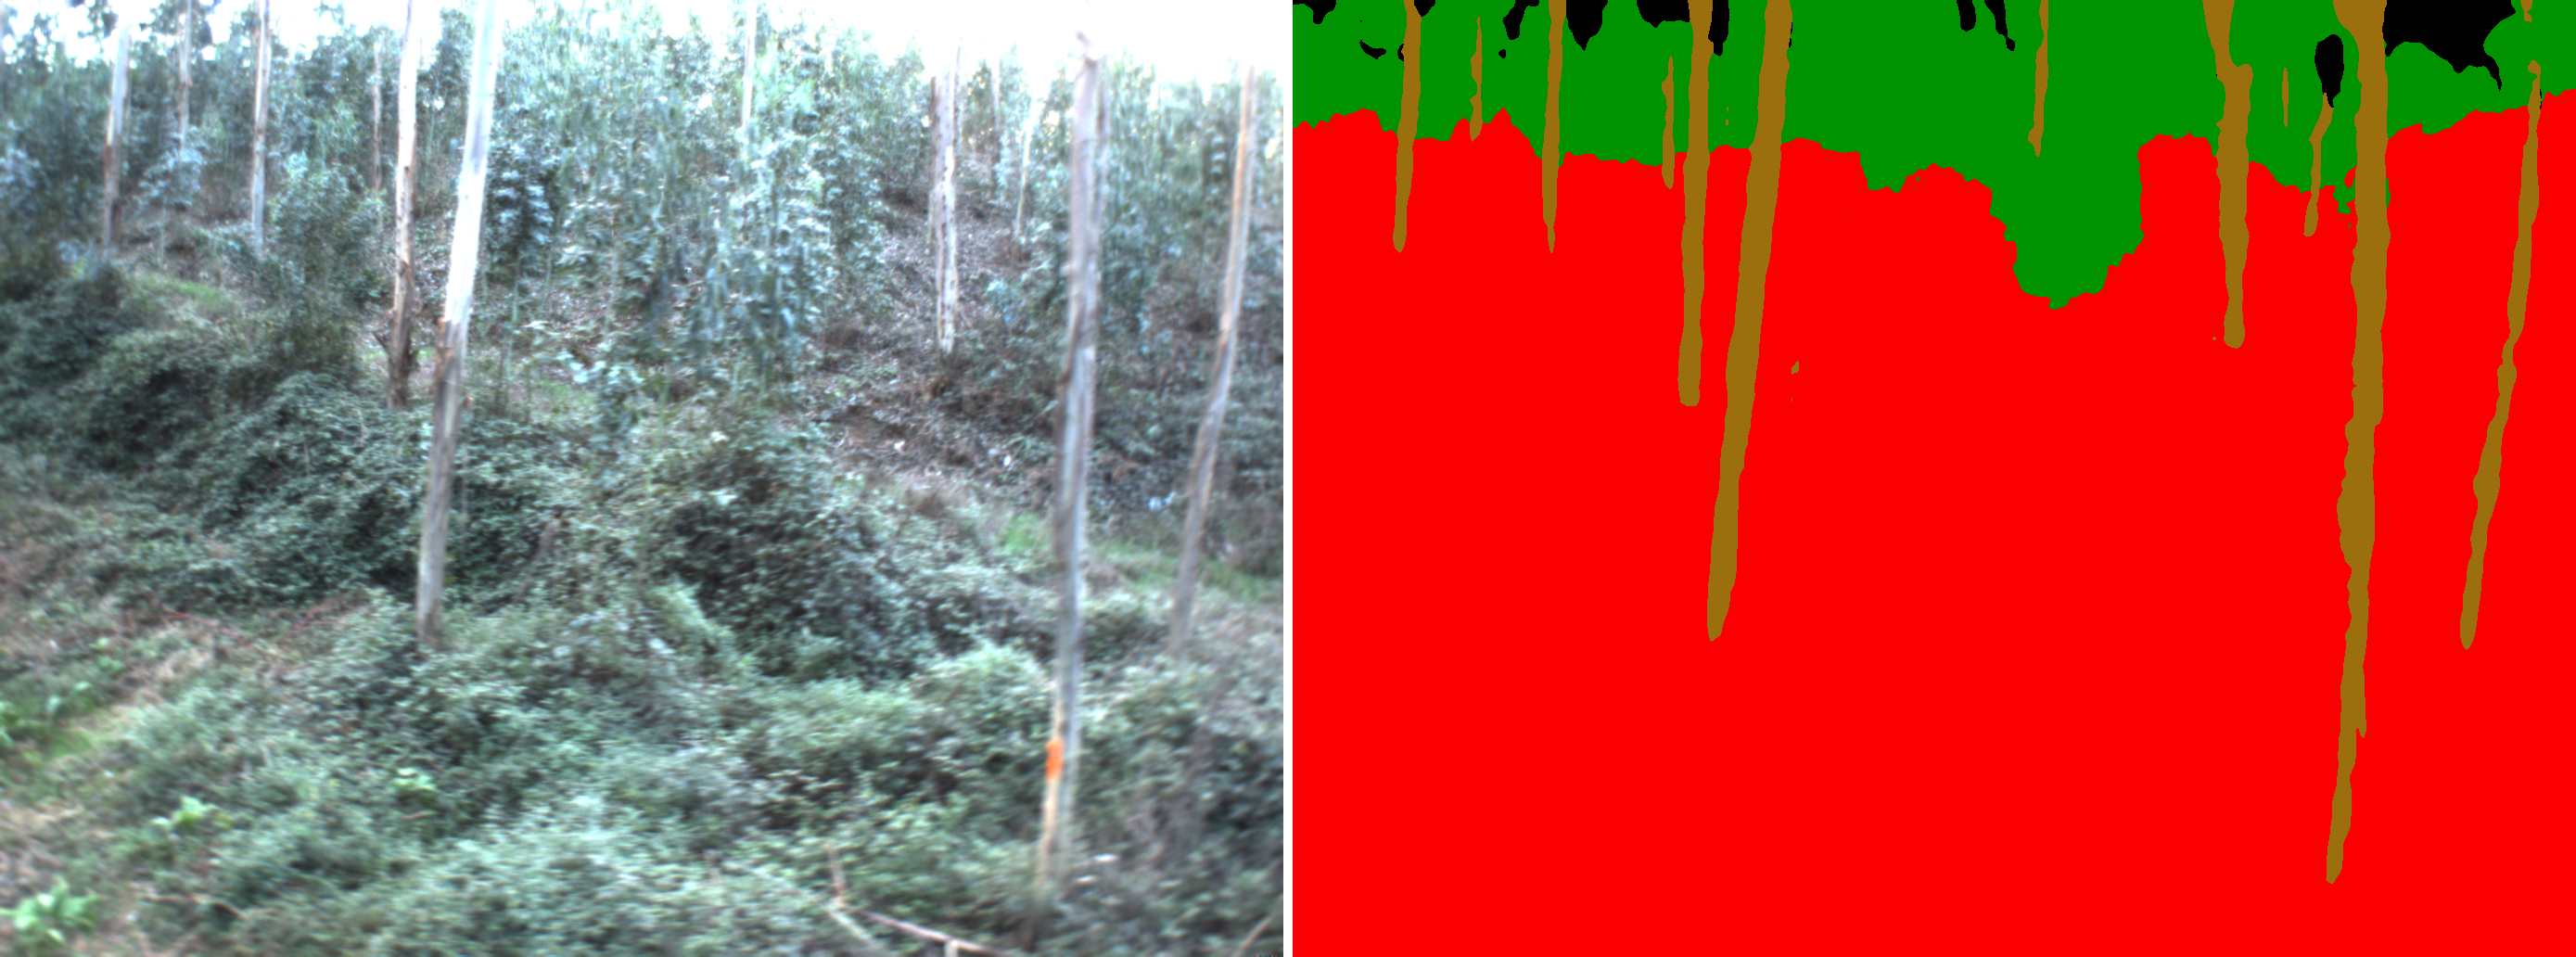
\includegraphics[width=\linewidth]{figs/results/semantic_segmentation/SeteFontes/qualatative_001600.png}  
    \caption{Predictions on the \textit{Oporto} dataset. Black is background, red is fuel, brown is trunks, and green is canopy.
    %Note that low trees are often predicted as fuel.
    } 
    \label{fig:qualitative_semantics_semfire}
\end{figure}

We conducted experiments to determine how many real training images were needed, with and without synthetic pretraining, as seen in Figure \ref{fig:quant_semantics}. We used mean Intersection over Union (mIoU) to evaluate the quality of the predictions on the test set. It is interesting to note the relatively high performance of a model that used only 7 real images. Also, the model trained solely on synthetic data fails to generalize to real data, even after properly accounting for differences in mean and variance of both datasets. We found that combined real and synthetic data performs worse than training the same model only using real data. This suggests that the synthetic data comes from a completely different distribution than the real one, making its contribution detrimental. In the future, we plan to keep researching the causes of this interesting outcome.

As the model trained in 121 images ($80\%$ of the \textit{Setes Fontes} dataset) showed the best performance and was used for deployment in the \textit{Oporto} dataset, which was never seen during training.
%Qualitative examples of both can be seen in Figure \ref{fig:qualitative_semantics_semfire} and
The confusion matrix on the \textit{Setes Fontes} test set can be found in Figure \ref{fig:semantics_confusion} and qualitative results are in Figure \ref{fig:qualitative_semantics_semfire}. As we are mainly interested in the fuel instances, we aggregated the background, trunks, and canopies in a single non-fuel class. In that case we obtained an IoU of 78.2\% and 95.3\% for \texttt{Fuel} and \texttt{Not Fuel}, respectively, which yields a mIoU of 86.7\%. This shows that our system performs well at its primary task of identifying fuel.





In our evaluation of the semantic segmentation model, we utilize a small annotated test set derived from the semantic mapping mission in the rural test site, which was not used for training. For this purpose, we annotated 17 images using the same strategy employed during training, but these images were not included in the training dataset. Similarly for the training case, it is worth to note that despite of having 17 images, the actual instances used for testing are higher. This is because some classes can appear more than once in a single image. We conducted an analysis of the semantic segmentation using precision, recall and intersection over union (IoU) metrics to assess the fuel classification in our system. These metrics were chosen because of their importance for addressing false positive/negative results while IoU estimates the general quality of the segmentation. 
% Our focus lied in assessing precision, recall, and Intersection over Union (IoU) specifically for the fuel classes that appear abundantly in this particular scenario.

It is worth noting that certain classes which were included in the original 15 classes, are absent from the evaluation Table \ref{tab:semantic_eval}. This is because these classes were not present in the test set, as seen in Figure \ref{fig:class_frac}.
Consequently, these classes were excluded from the results. There is a noticeable shift in performance between the common classes and the rare classes, which is unsurprising. However, since we aggregate these classes after predictions, the errors on the rare classes only have a small impact on the final aggregate predictions.

\begin{figure*}[h!]
   \centering
   %----primera subfigura----
   \subfloat[]{
        \label{fig:train_class_frac}         %% Etiqueta para la primera subfigura
        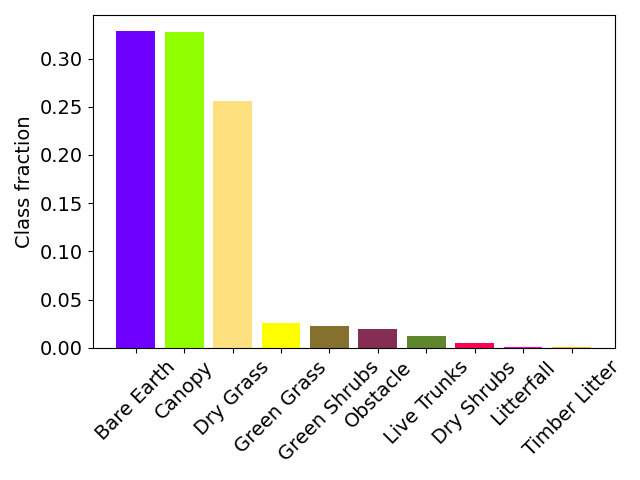
\includegraphics[width=0.5\textwidth]{figs/results/semantic_segmentation/class_fraction_train.png}}
   %\hspace{0.1\linewidth}
   \subfloat[]{
        \label{fig:test_class_frac}         %% Etiqueta para la segunda subfigura
        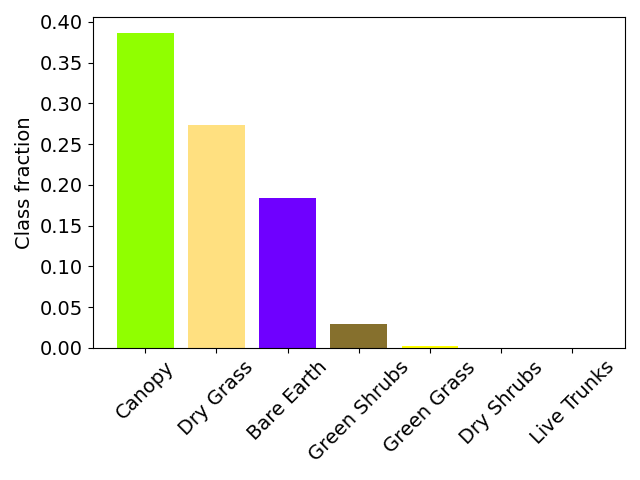
\includegraphics[width=0.5\textwidth]{figs/results/semantic_segmentation/class_fraction_test.png}}%\\[20pt]            
   \caption{This shows the fraction of pixels per class for A) the train set and B) the test set. Note that the three dominant classes Canopy, Bare Earth, and Dry Grass are common across both collections but the comparative frequencies are somewhat different. These correspond to our aggregate Canopy, Background, and Fuel classes respectively. The fractions of other classes are fairly small, and some from the training set are entirely absent in the test set.}
   \label{fig:class_frac}                %% Etiqueta para la figura entera
\end{figure*}


\begin{table}[ht!]
    \centering
\begin{tabular}{ccccc}
% \hline
\toprule
\textbf{Class} & \textbf{IoU} & \textbf{Precision} & \textbf{Recall} \\ \midrule
% \hline
Canopy & 70.05 & 84.77 & 80.13 \\
Dry Grass & 79.7 & 93.75 & 84.17 \\
Bare Earth & 78.53 & 88.12 & 87.83 \\
Green Shrubs & 3.27 & 21.72 & 3.71 \\
Green Grass & 0.0 & 0.0 & 0.0 \\
Dry Shrubs & 0.0 & 0.0 & 0.0 \\
Live Trunks & 0.05 & 0.05 & 84.09 \\
\bottomrule
% \hline
\end{tabular}
\caption{Evaluation results of the SegNext network with the Anderson Fuel Model as a base for semantic segmentation in a forestry environment.}
\label{tab:semantic_eval}
\end{table}


\begin{figure*}[h!]
   \centering
   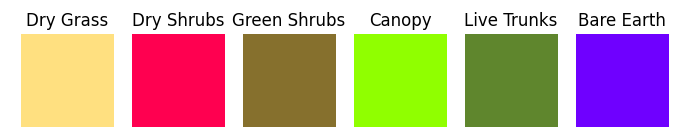
\includegraphics[width=0.5\textwidth]{figs/results/semantic_segmentation/Gascola/safeforest_all_classes_flat.png}
   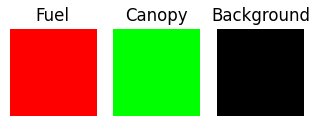
\includegraphics[width=0.25\textwidth]{figs/results/semantic_segmentation/Gascola/safeforest_classmap_compressed_flat.png}
   \includegraphics[width=0.80\textwidth]{figs/results/semantic_segmentation/Gascola/000000_rgb_img.png}
   \vspace{0pt}
   \includegraphics[width=0.80\textwidth]{figs/results/semantic_segmentation/Gascola/000005_rgb_img.png}
   \vspace{0pt}
   \includegraphics[width=0.80\textwidth]{figs/results/semantic_segmentation/Gascola/000010_rgb_img.png}
   \vspace{0pt}
   \includegraphics[width=0.80\textwidth]{figs/results/semantic_segmentation/Gascola/000015_rgb_img.png}
   \vspace{0pt}
   \caption{
   Qualitative semantic mapping results from the test set. The results are shown both for the predicted classes and the aggregated ones, with colors visualized in the top rows.
   White regions in the ground truth represent areas that were ambiguous to the human annotator. Overall the predictions match the ground truth well and boundaries are well-defined. Note that many regions of confusions, such as canopy-to-trunk and green shrub to canopy, fall within the same coarse classes for our mapping purposes.
   }
   \label{fig:results_semantic_seg_qualitative}                %% Etiqueta para la figura entera
\end{figure*}

\subsection{Projecting Segmentation into 3D}
The final goal of semantic mapping is to develop a model of the environment and what class different regions are. To evaluate the feasibility of this, we conduct two experiments using multi-sensor data.
The first experiment uses data that we collected under the canopy using a payload inclination of 30 degrees from horizontal. The drone was manually piloted to survey the perimeter of a clearing.  

\begin{figure}
    \centering
    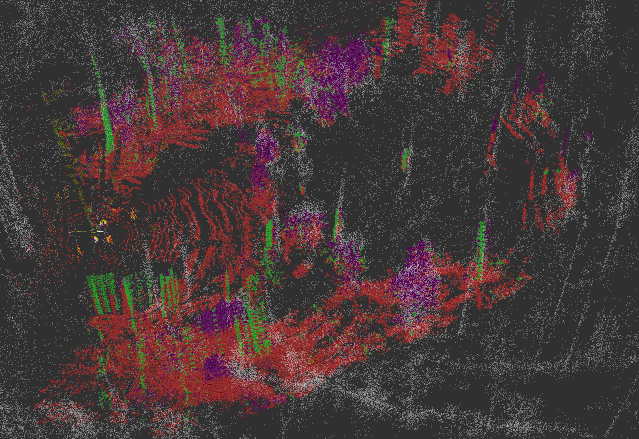
\includegraphics[width=0.8\textwidth]{figs/results/semantic_mapping/semantic_cloud_first_approach.png}
    \caption{Semantic mapping results on the Oporto test site. Fuel is red, trunks are green, canopy is purple, and background is black. White points are unlabeled.}
    \label{fig:semantic_SLAM_result}
\end{figure}

In our second experiment, we sought to evaluate the perfomance more rigorously. This is challenging because accurate field-reference data is challenging to acquire. Instead, we choose to label an orthomosoaic derived from a 3D model by hand. We did this using QGis\footnote{\url{https://qgis.org/en/site/}}, an open-source software for interacting with geospatial data. We labeled three coarse classes, fuel, canopy and background, which included bare-earth and other non-flammable material. This manual process took approximately eight hours to complete and is visualized on the left side of Figure \ref{fig:results:semantic_map_UFO}.


\begin{figure}
    \centering
    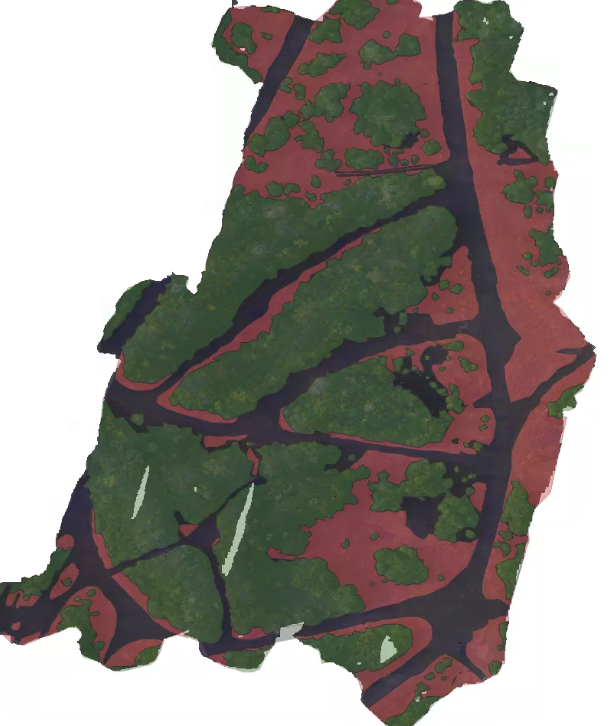
\includegraphics[width=0.45\textwidth]{figs/results/semantic_mapping/labeled_orthomoasaic.png}
    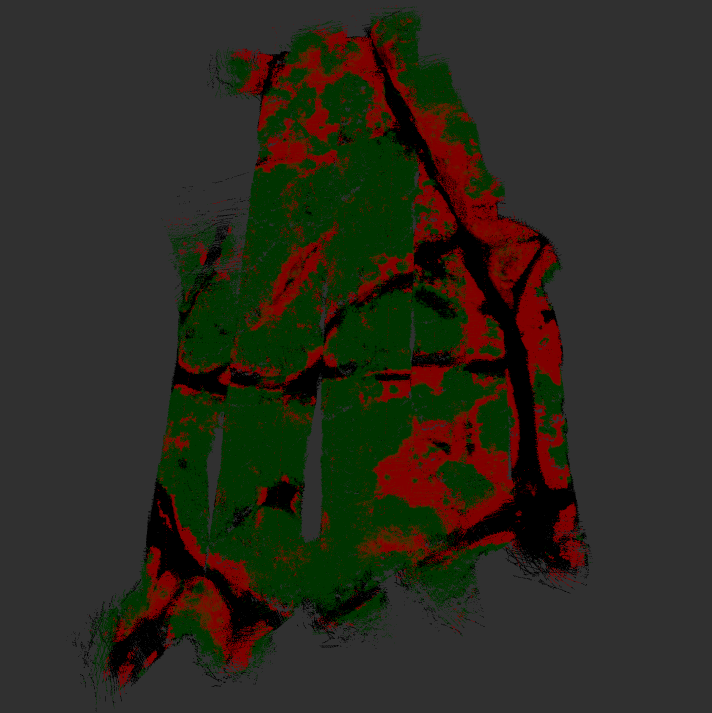
\includegraphics[width=0.45\textwidth]{figs/results/semantic_mapping/segnext_gc5_ufomap.png}
    \caption{Manually-labeled result on the left, result from UFO-Map on the right provided by M. Duda Andrada, using the semantic segementation model described previously. }
    \label{fig:results:semantic_map_UFO}
\end{figure}

\section{Tree detection}
Our work shows that the tree detection results are substantially better on drone data compared to NAIP as shown in Figure \ref{fig:results:tree_det}. However, the quality of NAIP detections can be improved substantially by finetuning the model on only a small amount of data.

\begin{itemize}
    \item TODO expand this
    \item TODO the most important figure to add is probably a table of metrics for the different approaches.
\end{itemize}

\begin{figure}[h]
    \subfloat{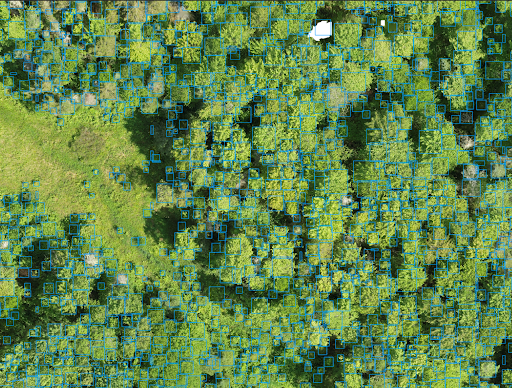
\includegraphics[width=0.45\textwidth]{figs/results/tree_detections/stowe_anew_base.png}}
    \hfill
    \subfloat{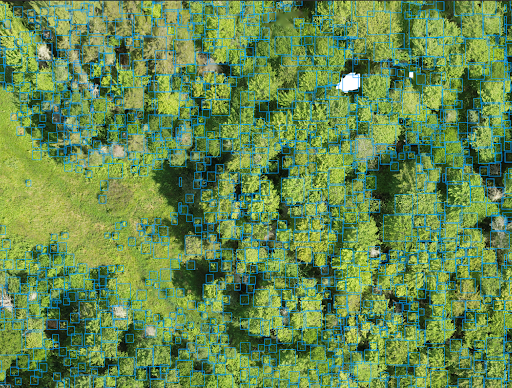
\includegraphics[width=0.45\textwidth]{figs/results/tree_detections/stowe_anew_retrained.png}}
    \vfill
    \subfloat{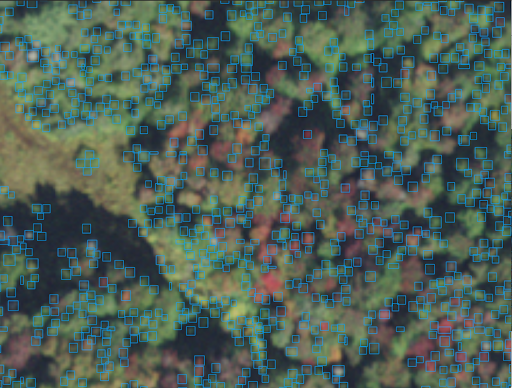
\includegraphics[width=0.45\textwidth]{figs/results/tree_detections/NAIP_base.png}}
    \hfill
    \subfloat{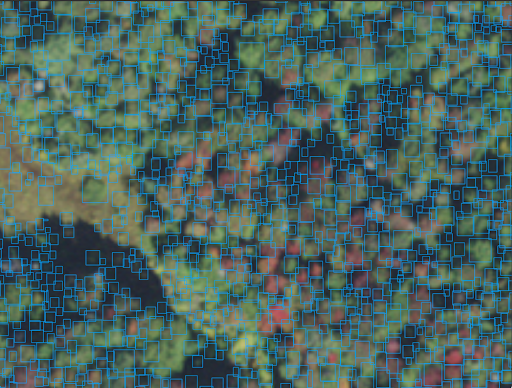
\includegraphics[width=0.45\textwidth]{figs/results/tree_detections/NAIP_retrained.png}}
    \caption{Tree detections on an orthomosiac (top) and NAIP data (bottom). The left column shows the DeepForest predictions without any retraining, while the right column shows the results after retraining on a small amount of local annotations.}
    \label{fig:results:tree_det}
\end{figure}

\section{Informative path planning}

\begin{figure}[h]
    \subfloat{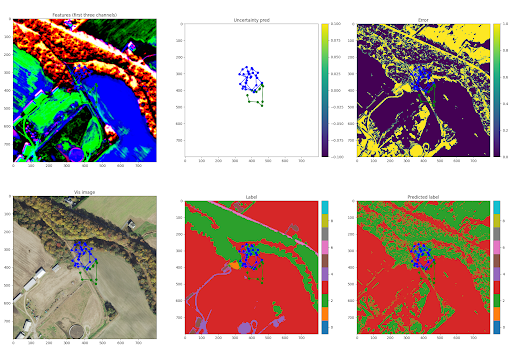
\includegraphics[width=0.45\textwidth]{figs/results/ipp/unpaired_qual_1 (1).png}}
    \hfill
    \subfloat{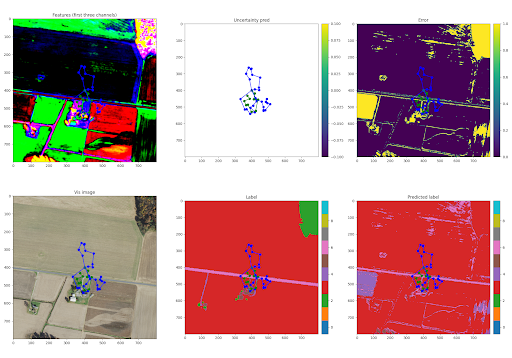
\includegraphics[width=0.45\textwidth]{figs/results/ipp/unpaired_qual_2 (1).png}}
    \caption{Visualizations of the proposed planning method on two different data images.}
    \label{fig:res_unpairqual}
\end{figure}


\begin{figure}[h]
    \subfloat{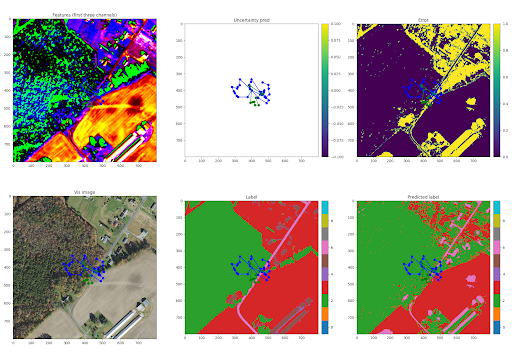
\includegraphics[width=0.45\textwidth]{figs/results/ipp/paired_qual_GBS-IPP (1).png}}
    \hfill
    \subfloat{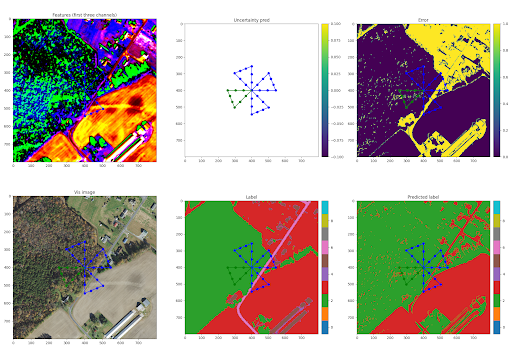
\includegraphics[width=0.45\textwidth]{figs/results/ipp/paired_qual_pizza (1).png}}
    \caption{A comparison of the proposed method with a baseline}
    \label{fig:res_pairedqual}
\end{figure}

\begin{figure}[h]
    \subfloat{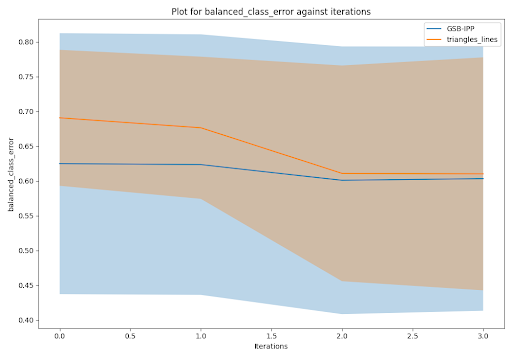
\includegraphics[width=0.3\textwidth]{figs/results/ipp/error (2).png}}
    \hfill
    \subfloat{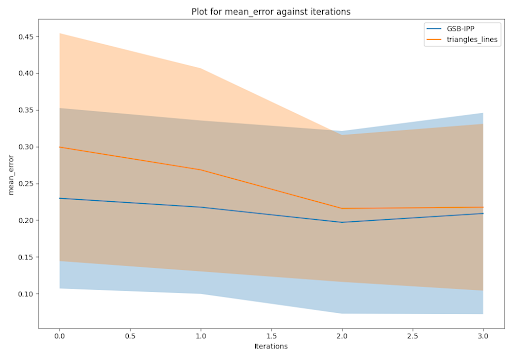
\includegraphics[width=0.3\textwidth]{figs/results/ipp/balanced_error (2).png}}
    \hfill
    \subfloat{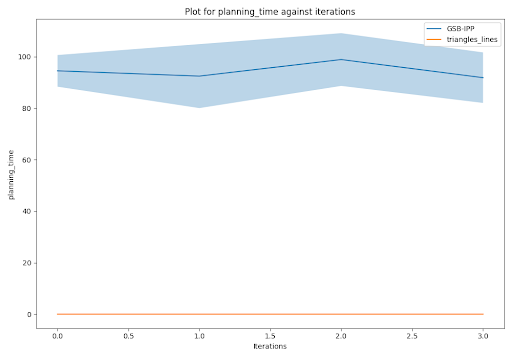
\includegraphics[width=0.3\textwidth]{figs/results/ipp/timing_result (1).png}}
    \caption{Quantitative statistics for IPP. TODO replace with updated ones.}
    \label{fig:res_ipp_quant}
\end{figure}

\subsection{Problem formulation}
The goal of the experiments is to model a realistic data collection scenario. The data is collected over a series of missions, where each mission must be fully planned before it is executed. Each mission is allowed a pathlength budget and a number of samples it is allowed to collection. 

In our experiments we use randomly-sampled NAIP tiles to evaluate the approach. In each situation the agent starts in the center of the environment and must return there after each mission.

In these experiments we use a very simple prediction system to predict the class of unobserved pixels. It is simply a nearest-neighbor classifier which operates on the same PCA-compressed MOSAIKS features that are used for planning. While simple, this approach is well-suited to the extremely low number of training samples used in this setting and the standardized and uncorrelated nature of our feature space.

Before any missions have been executed, the agent can only observe the label of the pixel it is at. Then it plans a mission and executes it, observing the labels at the chosen sampling locations. These samples are used to train a prediction model which is used for evaluation and, in theory, could be used to inform the plan for the next mission. 


The experiments were conducted over ten random domains, which each represented an 800x800px crop from the Chesapeake Bay land cover dataset. Each tile represents approximately half a kilometer square. The pathlength was set as 800 pixels as well, which meant that the agent could go to one side of the environment and return to the start within the budget but some corners were completely unreachable. Each domain was explored using four missions where 10 samples could be collected during each one. Each sample meant the agent could observe the class of one pixel. After each mission, the class of all pixels  were predicted using the nearest neighbor classifier and the error metrics were computed. 


\subsection{Metrics}
The quality of the predictions are evaluated on two metrics, accuracy and averaged recall. The first is simply the fraction of pixels in the map that were assigned the correct class label by the prediction system. The second represents the average of the per class recalls. This metric is chosen so that rare classes are treated equally in the evaluation procedure, since this is critically important when we explicitly want to find rare classes. We also report the time taken to generate the plan. Note that this does not include the time taken to generate the class predictions, since the planner is agnostic to the choice of prediction algorithm.



